\documentclass[a4paper,12pt]{article}

\usepackage{amsmath}
\usepackage{graphicx}
\usepackage{color}
\usepackage{hyperref}
\hypersetup{
    colorlinks=false,
    linkcolor=blue,
    }
\begin{document}
\title{\textbf{CSE 376: Technical Writing and Presentation}}
\author{Naimul Hasan}
\date{\today}
\maketitle
\pagenumbering{roman}
\tableofcontents
\newpage
\pagenumbering{arabic}

\section{Checkpoint 01}
\subsection{Introduction}
I'm Naimul Hasan. I am a 3rd year student studying Computer Science and
Engineering at Shahjalal University of Science \& Technology.
\subsection{Courses}
\subsubsection{Object-oriented programming}
\label{stage1}
In this course i have learnt a famous object oriented language called Java.
\subsubsection{Data structures and algorithms}
In this course i have learnt many algorithms and data structures.
\subsection{Projects}
I have done a project in this \ref{stage1} course.

\newpage
\section{Checkpoint 02}
\subsection{Font Effects}
\textit{The text in italics} \\
\textsl{The text in slanted} \\
\textsc{The text in smallcaps} \\
\textbf{The text in bold} \\
\texttt{The text in teletype} \\
\textsf{The text in sans serif} \\
\textrm{The text in roman words} \\
\underline{The text in underlined words} \\

\subsection{Coloured Text}
{\color{green}Green},
{\color{blue}blue},
{\color{cyan}cyan},
{\color{magenta}magenta},
{\color{red}red},
{\color{yellow}yellow}
\\
\subsection{Font Sizes}
Different font sizes in \LaTeX \\

{\tiny This text is tiny words} \\

{\scriptsize This text is in scriptsize words} \\

{\footnotesize This text is in footnotesize words} \\

{\small This text is in small words} \\

{\normalsize This text is in normalsize words} \\

{\large This text is large words} \\

{\Large This text is Large words} \\

{\LARGE This text is LARGE words} \\

{\huge This text is huge words}


\subsection{Lists}
Item in the menu
\begin{enumerate}
    \item Rice
    \item Lentil soup
    \item Vegetables
    \begin{itemize}
        \item Cabbage
        \item Bottle gourd
        \item Cauliflower
        \item String bean
    \end{itemize}
    \item Beef
    \item Fish
    \begin{itemize}
        \item Katla
        \item Rui
    \end{itemize}
\end{enumerate}
\subsection{Comments \& Spacing}
I have done some comment here though it is not showing in the pdf %this text will not be shown as it is comment 
\\    After some               space.

\subsection{Special Characters}
Item \#1A\textbackslash 642 costs \$8 \& is sold at a \~{}10\% profit.
 
\newpage
\section{Checkpoint 03}
\begin{tabular}{l|r|r}
    Item & Quantity & Price(\$) \\
    \hline
    Nails & 500 & 0.34 \\
    Wooden boards & 100 & 4.00 \\
    Bricks & 240 & 11.50 \\
\end{tabular}
\newline
\vspace{24pt}
\newline
\begin{tabular}{l|ccc}
     & \multicolumn{3}{c}{Year} \\
    \cline{2-4}
    City & 2006 & 2007 & 2008 \\
    \hline
    London & 45789 & 46551 & 51298 \\
    Berlin & 34549 & 32543 & 29870 \\
    Paris & 49835 & 51009 & 51970 \\
\end{tabular}
\newpage


\section{Checkpoint 04}
\begin{figure}[h]
    \centering
    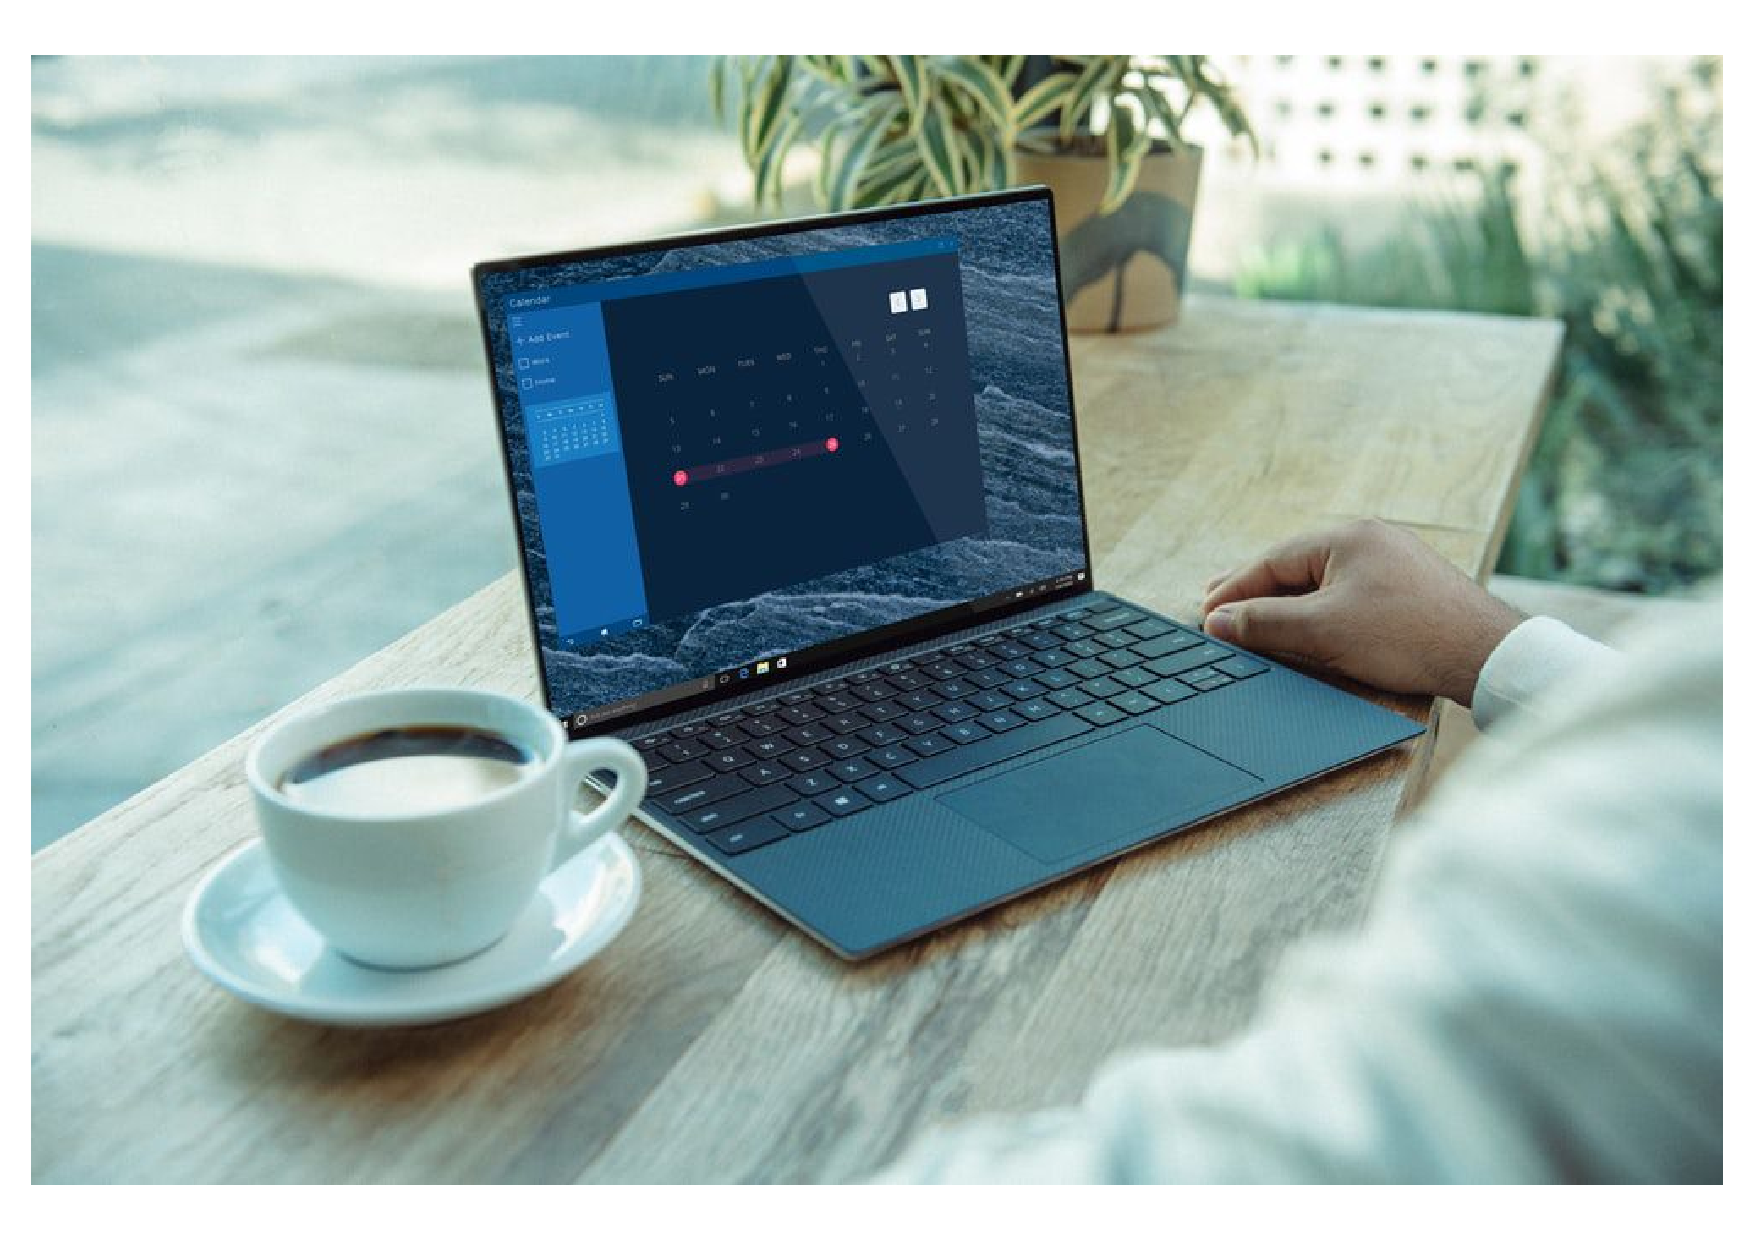
\includegraphics[width=1\textwidth]{myimage}
    \caption{Coffee during work}
    \label{fig:my_label}
\end{figure}
\newpage

\section{Checkpoint 05}
\begin{eqnarray}
    e = mc^2 \\
    \pi = \frac{c}{d} \\
    \frac{d}{dx}e^x = e^x \\
    \frac{d}{dx}\int_0^\infty f(s)ds = f(x) \\
    f(x) = \sum_i = 0^\infty\frac{f^{(i)}(0)}{i!}x^i \\
    x = \sqrt{\frac{x_i}{z}y} \\
     \left[
    \begin{matrix}
      1 & 2 & 3 & 4 & 5 \\
      6 & 7 & 8 & 9 & 10 \\
      11 & 12 & 13 & 14 & 15 \\
      16 & 17 & 18 & 19 & 20 \\
      21 & 22 & 23 & 24 & 25 \\
    \end{matrix}
    \right]
\end{eqnarray}

\newpage
\section{Checkpoint 06}
Some references from the review assignment.
\cite{ahmed2014protibadi}
\cite{ahmed2015learning}
\cite{bardzelland}
\cite{bardzell2010feminist}
\cite{brewerbowei}
\cite{burrell2010evaluating}
\cite{butler2011bodies}
\cite{chen2015computing}
\cite{chess2015conspiracy}
\cite{clark2005women}
\cite{corbin1990grounded}
\cite{dimond2013hollaback}
\cite{halder2011cyber}
\cite{haraway2006cyborg}
\cite{houston2016values}
\bibliographystyle{plain}
\bibliography{references} 
\end{document}
